\section{Computing error in specific observables}




\subsection{Assessing quality of data}
%    - Data filtering [Paul]
Generally speaking, analysis routines that extract derived quantities from raw data are often formulated on the basis of physical intuition about how that data should behave.  Before proceeding to data analysis, it is therefore useful to assess the extent to which raw data conforms to these expectations and the requirements imposed by the analysis routines.  Such tasks help reduce subjectivity of predictions and offer insight into when a simulation protocol should be revisited to better understand their meaningfulness \cite{patrone1}.  Unfortunately, general recipes for assessing data quality are impossible to formulate, owing to the range of physical quantities of interest to modelers.  Nonetheless, a short example will help clarify the matter.

In the context of materials science, understanding when a structural material fails is critical for many engineering applications.  In the past decade, scientists have increasingly focused on modeling the yield-strain $\epsilon_y$, which is (loosely speaking) the amount of stretching (or strain) at which it deforms irreversibly.  Intuition and experiments tells us that upon deforming a material by a fraction $1+\epsilon$, it should recover its original dimensions if $\epsilon \le \epsilon_y$ and have a residual strain $\epsilon_r = \epsilon - \epsilon_y$ if $\epsilon \ge \epsilon_y$ \cite{patrone2}.  Owing to the time-scale limitations of MD, it is also reasonable to expect that the transition in $\epsilon_r$ around yield will be smooth and not piecewise linear.  Thus, if we fit residual strain to a hyperbola, the proximity of data to the asymptotes illustrates the extent to which simulated $\epsilon_r$ conforms to the expectation that $\epsilon_r=0$ when $\epsilon < \epsilon_y$.  See Fig.~\ref{fig:yield}.

\begin{figure}
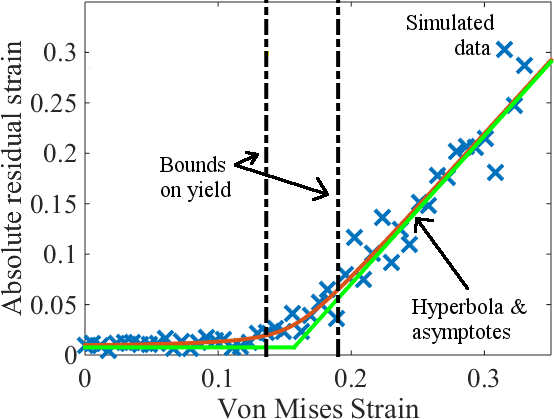
\includegraphics[width=8cm]{hyperbola.png}\caption{Yield strain tn $\epsilon_r$ as a function of applied strain $\epsilon$.  Blue $\times$ denote simulated data, whereas the smooth curve is a hyperbola fit to the data.  The green lines are asymptotes; their intersection can be taken as an estimate of $\epsilon_y$.    Bounds on yield are computed by the synthetic data method discussed in the next section.}\label{fig:yield}
\end{figure}

\subsection{Block averaging}
[Dan Z/Alan?/Dan S] Flyvjberg and Petersen 

\subsection{Propagation of uncertainty}

The quantities we are most interested in may not be simulation observables.  For instance, the free energy difference between two states might be measured by free energy perturbation, expressed as a function of the average of another quantity.
\begin{equation}
\beta \Delta A = -\ln \left< \exp \left(-\beta \Delta U\right) \right>
\end{equation}
Although $\exp(-\beta \Delta U)$ can be measured during the simulation and its uncertainty can be estimated directly using block averages as described above, $\beta \Delta A$ cannot be handled the same way.  If we compute $\beta \Delta A$ for each block, the values will tend to take extremely positive whenever the perturbation does poorly (where $\Delta U$ is consistently large).  In the pathological case, $\Delta U$ might be $\infty$ for every sample in a block and the $\beta \Delta A=-\ln 0$ cannot be computed. Instead of using block averages for $\beta \Delta A$, its uncertainty can be expressed as a first-order Taylor series expansion
\begin{equation}
  \sigma_{\beta \Delta A} = \sigma_{\exp(\beta \Delta U)} / \left< \exp \left(-\beta \Delta U\right) \right>
  \label{eq:propagation_bDA}
\end{equation}

Propagation of uncertainty is needed whenever the derived quantity can be expressed only as a function of other averages.  It might also be needed when the derived quantity is of a function of quantities measured in separate simulations, such as $<U(T_2)>-<U(T_1)>$.  If a derived quantity is a function of multiple observables measured within a single simulation, then terms must be included to account for the correlation between those observables.

Finally, because this approach is based on a first-order Taylor series, propagation of uncertianty can fail in cases where a non-linear formula is used and the uncertainty is very large.  For instance, the uncertainty in $\beta \Delta$ as prescribed by Eq.~\ref{eq:propagation_bDA} cannot exceed one no matter how short the simulation is or how bad the sampling is.  In such cases, it is necessary to use an alternate way to estimate the uncertainty or to simply use a different approach to compute the quantity of interest.

%[need a reference here.  I use https://en.wikipedia.org/wiki/Propagation_of_uncertainty but would be happy to cite a book or article that discusses basis for approach, handling complicated cases (covariance) and lists formulas for common cases]

\subsection{Bootstrapping}

In some cases, a derived quantity cannot be expressed as a function of the measured simulation data.  In such cases, bootstrapping may be able to yield an uncertainty \cite{EfronTibshiraniBootstrap}.  In simple bootsrapping, new data sets (corresponding to hypothetical simulation runs) are generated that consist of the samples that were generated during the actual run.  The set is generated with replacement (the same sample may be selected twice, others may not be selected at all), so each set will be different even though each is pulled from the same pool of data and contains the same number of samples.  Having created a new set, the data is analyzed to determine the derived quantity of interest.  This process is repeated to produce multiple estimates of the quantity; the uncertainty is the standard deviation of the computed quantities from the generated sets.

An alternate bootstrapping approach is called parametric bootstrapping.  Instead of selecting a new data samples from existing samples, new data are generated with some dependence on a parameter.  This is most useful to generate new average estimates from a Gaussian distribution centered at the nominal average with width equal to the uncertainty.  As with the simple bootstrap, the generated data can be used to compute the derived quantity of interest, and the uncertainty can obtained from the standard deviation of the values compute with different generated sets.

\subsection{Synthetic data models}
 %  - Generate synthetic data with noise model [Paul]
 
In certain cases, the transformation from raw data $\rho$ to a corresponding derived observable $F[\rho]$ may involve a non-linear operator that cannot reasonably be approximated by a Taylor series.  In such cases, numerical uncertainty propagation methods based on analysis of synthetic data can be useful.  

The main idea behind such approaches is to model the raw data $\rho$ as a deterministic ``trial'' function (which has free parameters) plus additive noise \cite{patrone1,patrone2,patrone3}.  The structure of the noise (for example, its covariance) can be inferred by (i) performing a best-fit of the trial function to the original data, and (ii) estimating the statistical properties of the noise on the basis of the residuals.  Having calibrated the noise model, random number generators can be used to sample the noise, which is then added back to the trial function to generate a synthetic data set.  As the task of generating synthetic data is inexpensive, one can often analyze many [e.g. $\mathcal O(10^5)$ or more] such sets in order to model the statistical properties.  See, e.g.\ Refs.~\cite{patrone1,patrone2,patrone3} for examples and practical implementations of such approaches.  


\subsection{Dark uncertainty analyses}
%- ‘Dark uncertainty’ analysis [Paul]

In some cases, multiple simulations of the same physical observable $\tau$ may yield predictions whose error bars do not overlap.  This situation can arise, for example, in simulations of the glass transition temperature when undersampling the crosslinked network structure of certain polymers.  In such cases, it is reasonable to postulate an unaccounted for source of uncertainty, which we colorfully refer to as ``dark uncertainty.''  In the context of a statistical model, we postulate that the probability of a simulation output depends on the unobserved or ``true'' mean value $\bar \tau$, an uncertainty $\sigma_i^2$ whose value is specific to the simulation (estimated, e.g.\ according to uncertainty propagation), and the unaccounted-for dark uncertinty $y^2$.  (For simplicity, the $\sigma_i^2$ and $y^2$ should be treated as variances.)  

While details are beyond this scope of this document, such a model motivates an estimate of $\bar \tau$ of the form 
\begin{align}
\bar \tau \approx \mathcal T \propto \sum_i \frac{T_i}{\sigma_i^2 + y^2}, \label{eq:darkmean}
\end{align}
where $T_i$ is the prediction from the $i$th simulation, $\sigma_i^2$ is its associated ``within-simulation'' uncertainty, and $y^2$ is the dark or between-simulation uncertainty; note that the latter does not depend on $i$.  The variable $y^2$ can be estimated from a maximum-likelihood analysis of the data and amounts to numerically solving a relatively simple nonlinear equation (see Ref.~\cite{patrone1}).  Equation~\eqref{eq:darkmean} is useful insofar as it weights simulated results according to their certainty while reducing the impact of overconfident predictions (e.g. having small $\sigma_i^2$).  Additional details on this method are provided in Ref.~\cite{patrone1} and the references contained therein.



- Basics: how to report, what goal to shoot for, significant figures
- When should you not trust uncertainties
    - Unknown unknowns
- If calculating a derived quantity, consider error in conversion from raw data 
    - Propagation of error (this doesn’t mean publishing your results!)
    - Taylor series expansion can handle cases where derived quantity is a direct function of measured data
    - Wikipedia: Propagation of uncertainty
    - Bootstrapping [Andrew/Dan S]
used for cases where the derived quantity is not simple function of the measured data.
An Introduction to the Bootstrap
    - Need to know correlation to correctly estimate sample size
    - Otherwise just gives relative uncertainty
- Correlation time analysis [Dan Z]
- Block averaging [Dan Z/Alan?/Dan S] Flyvjberg and Petersen 
- MOST OF THESE ALGORITHMS FAIL IF THE TRAJECTORY IS WAY TOO SHORT
    - If you miss the timescale by enough, you can’t tell
    - YOU HAVE TO THINK ABOUT THIS IN ADVANCE
- Link out to transport doc
